\chapter{Maquettes de projets}
\vspace{5cm}
\large{Ce quatrième chapitre est réservé à présentation des maquettes de projets.\\}


\newpage
\section{Maquette}
Une maquette est une représentation partielle ou complète d'un Système ou d'un objet (existant ou en projet) afin d'en tester et valider certains aspects et/ou le comportement (maquette fonctionnelle), ou simplement à des fins ludiques (maquette de jeu) ou informatives (présentation pédagogique ou commerciale d'une réalisation
ou d'un projet). Dans ce qui suit nous allons présenter les maquettes principales de notre site web .

\subsection{Maquette 1}
\begin{page}{\textwidth}
	\begin{page}{\linewidth}
	\makebox[\linewidth]{
		\includegraphics[keepaspectratio=true,scale=0.42]{Page_1.png}} 
		\captionof{figure}{Page d'acceuil}\label{f3}%
\end{page}
\end{page}

\subsection{Maquette 2}
\begin{page}{\textwidth}
	\begin{page}{\linewidth}
	\makebox[\linewidth]{
		\includegraphics[keepaspectratio=true,scale=0.42]{Page_3.png}} 
		\captionof{figure}{Créer un compte}\label{f3}%
\end{page}
\end{page}

\subsection{Maquette 3}
\begin{page}{\textwidth}
	\begin{page}{\linewidth}
	\makebox[\linewidth]{
		\includegraphics[keepaspectratio=true,scale=0.57]{Page_2.png}} 
		\captionof{figure}{Se connecter}\label{f3}%
\end{page}
\end{page}
\subsection{Maquette 4}
\begin{page}{\textwidth}
	\begin{page}{\linewidth}
	\makebox[\linewidth]{
		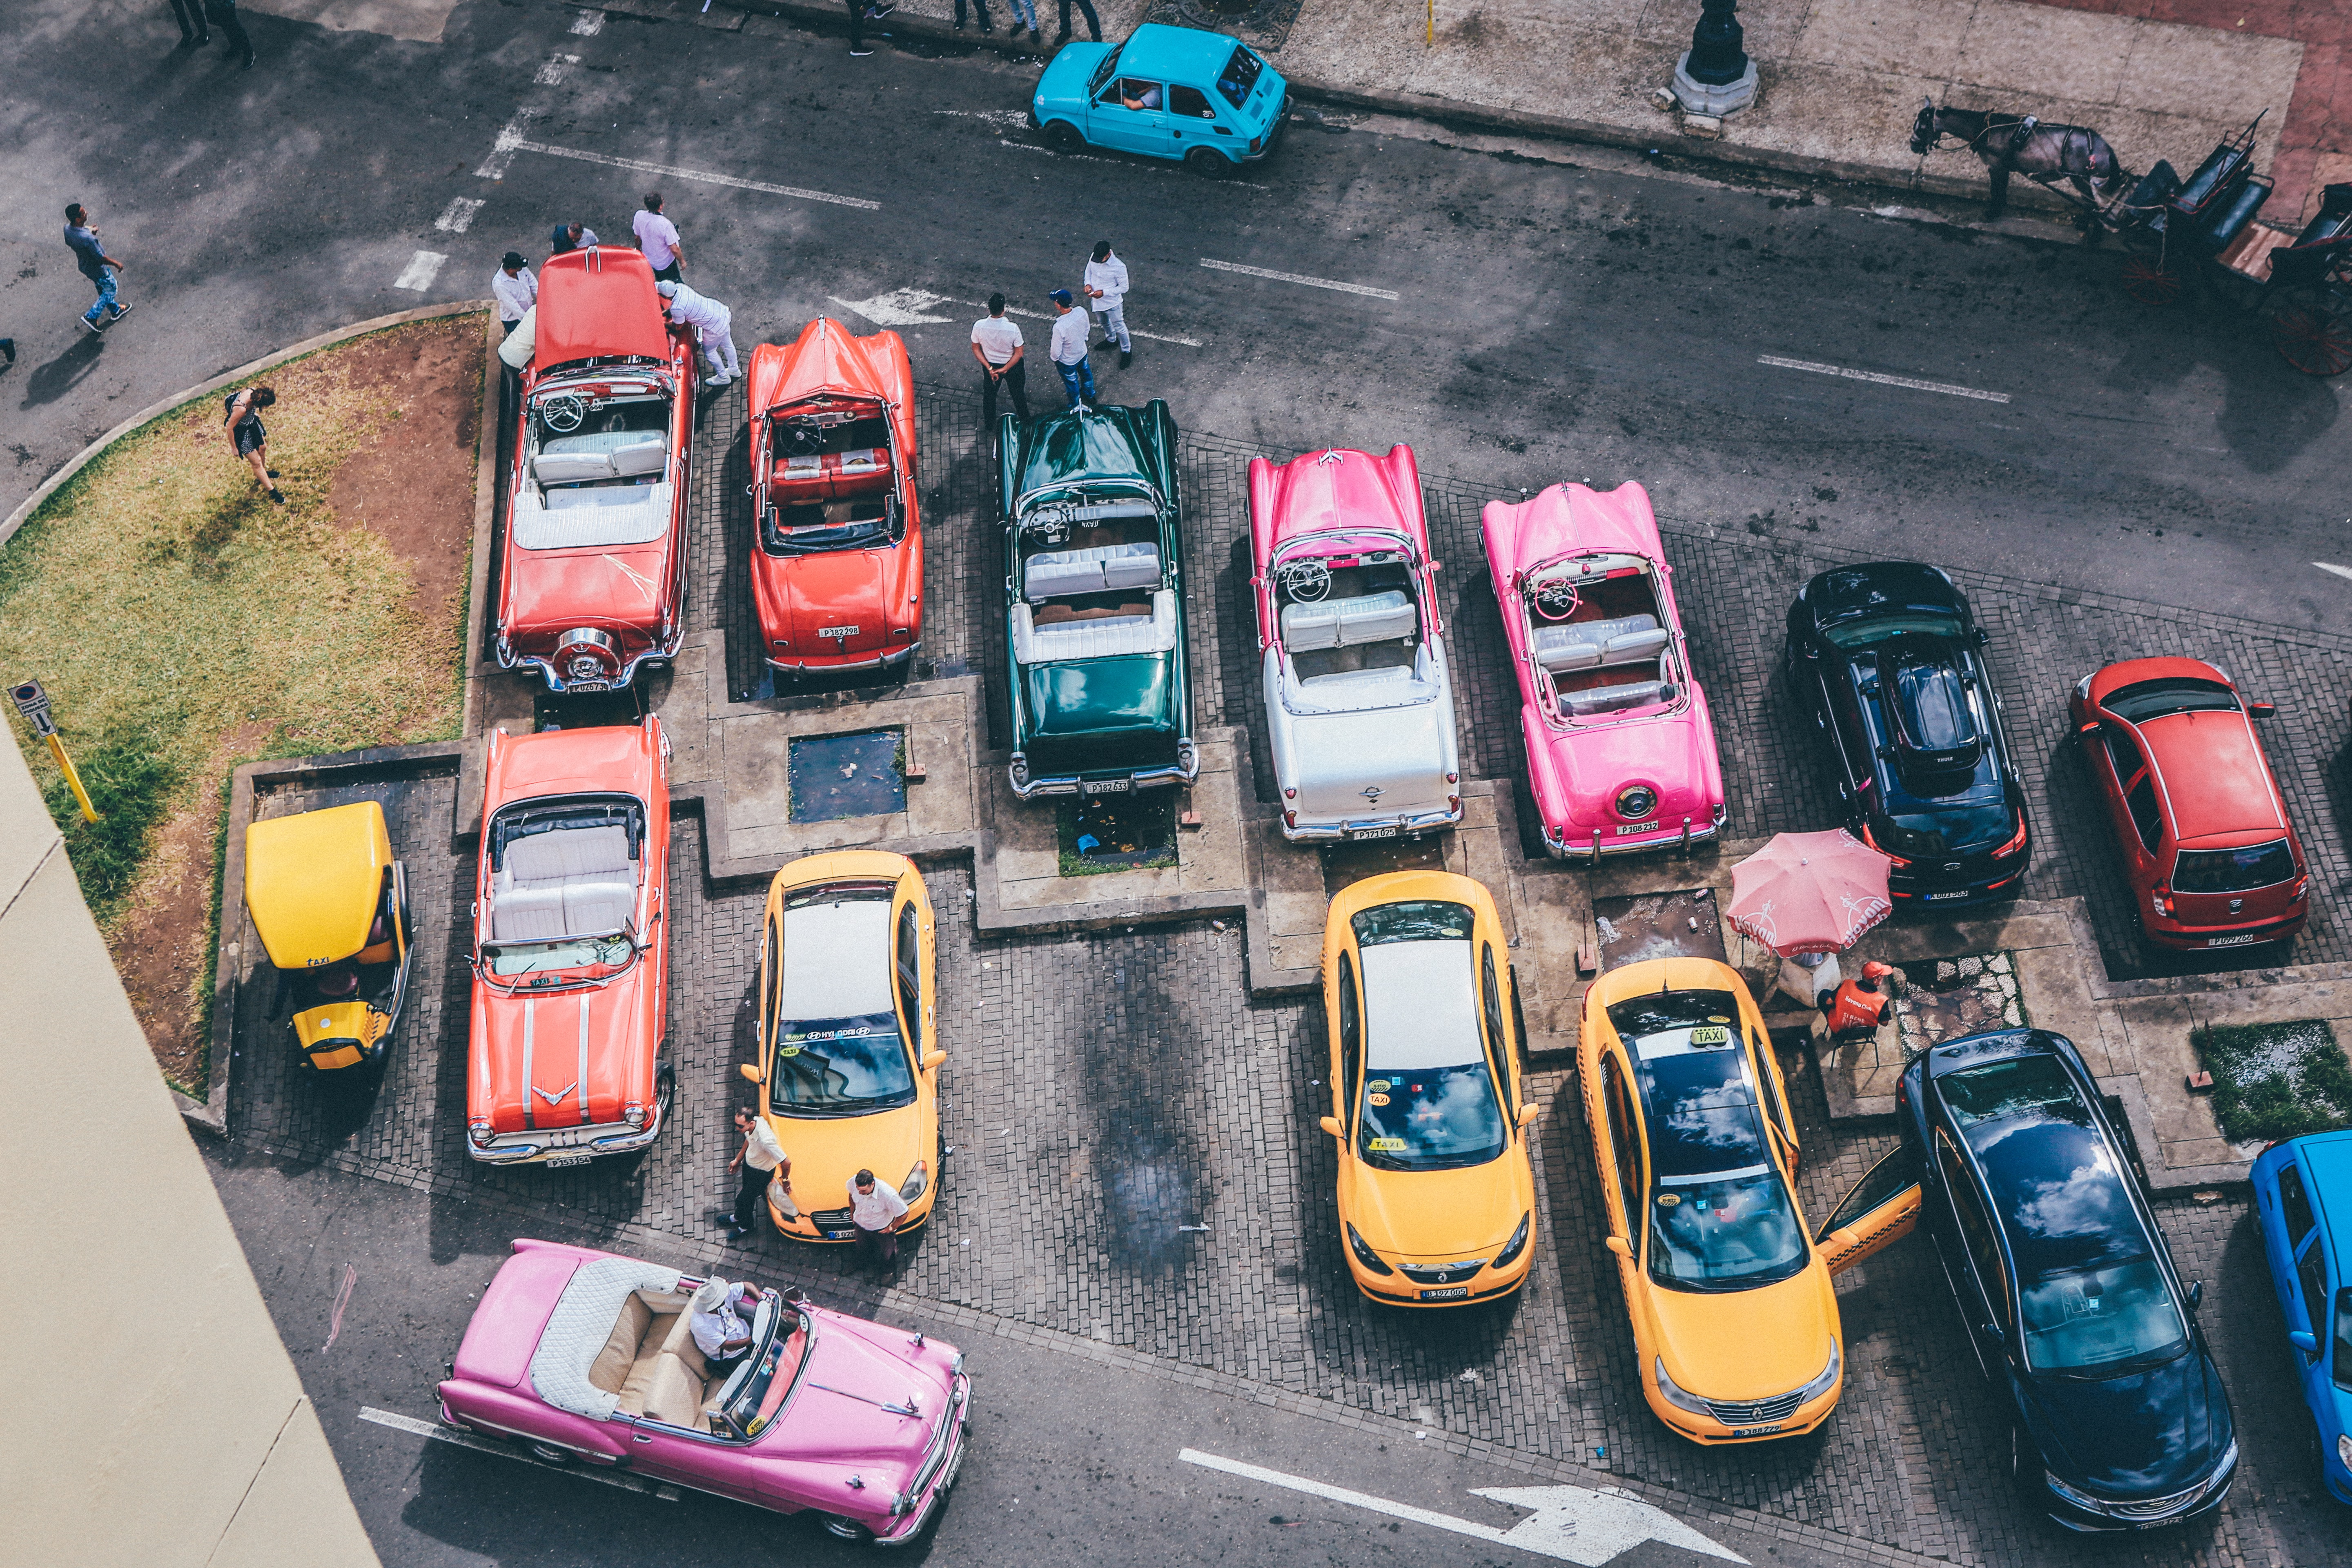
\includegraphics[keepaspectratio=true,scale=0.38]{1.png}} 
		\captionof{figure}{Page des offres}\label{f3}%
\end{page}
\end{page}
\subsection{Maquette 5}
\begin{page}{\textwidth}
	\begin{page}{\linewidth}
	\makebox[\linewidth]{
		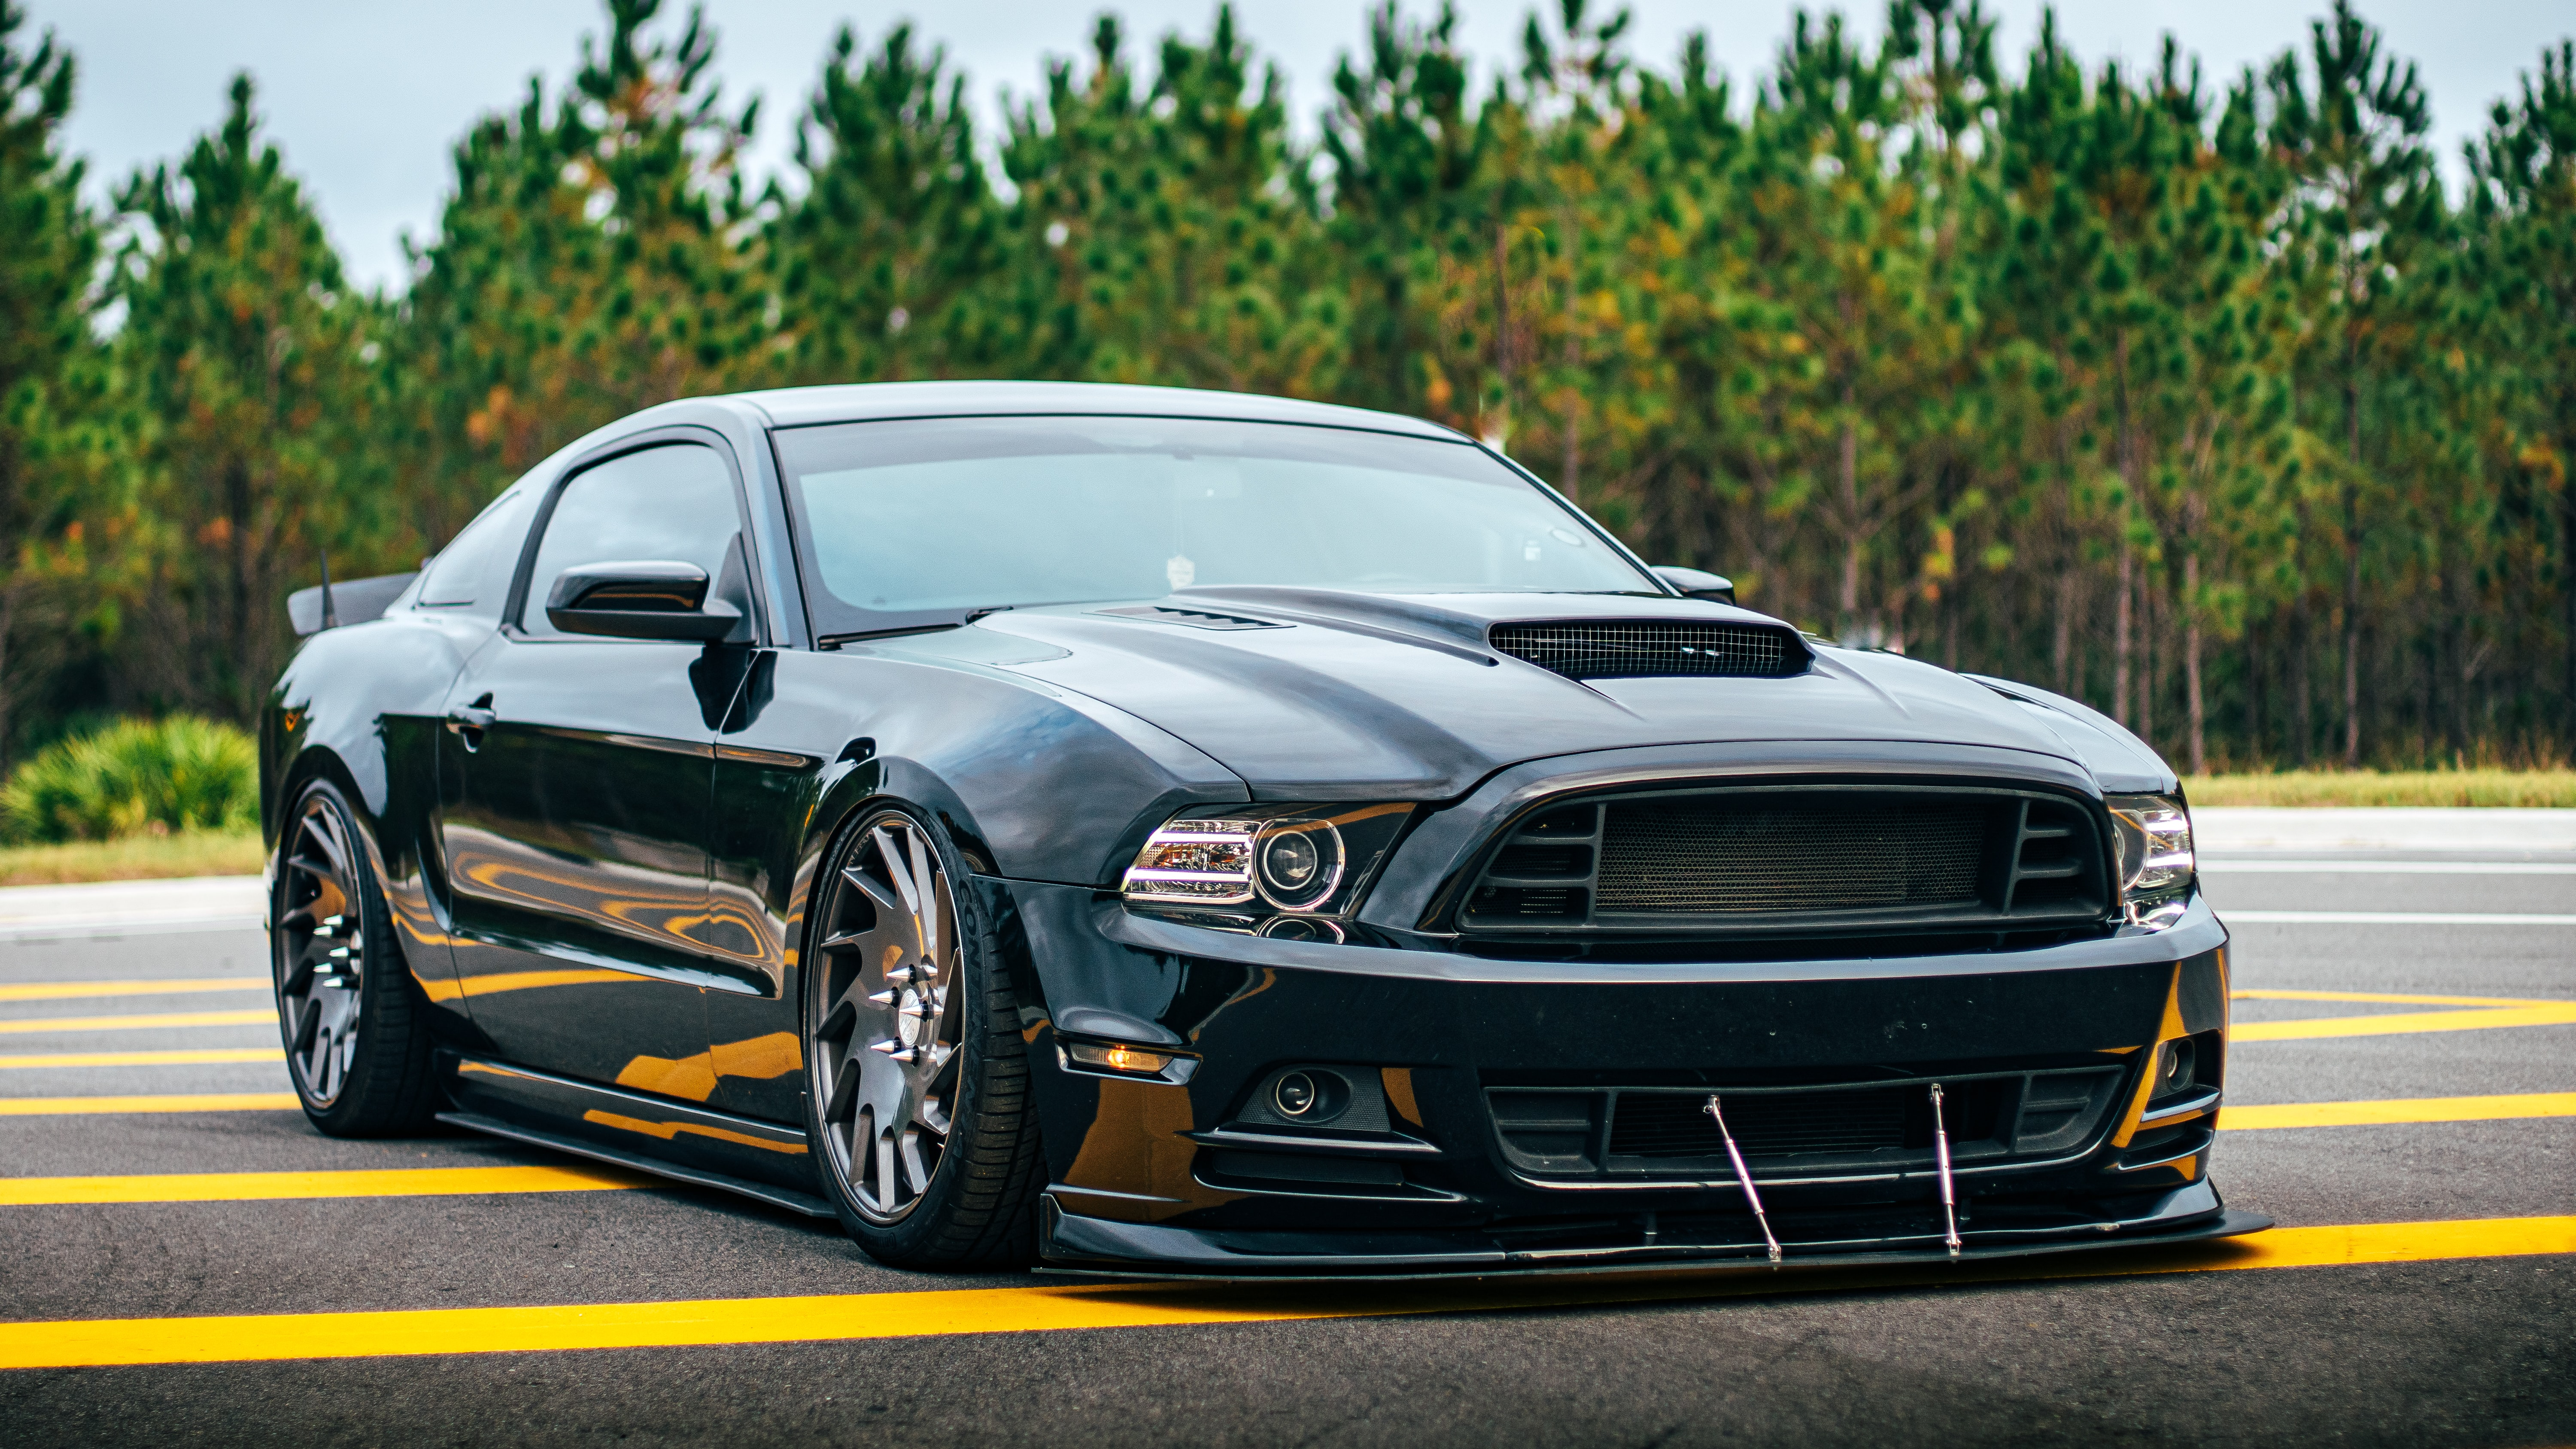
\includegraphics[keepaspectratio=true,scale=0.38]{2.png}} 
		\captionof{figure}{Description d'une offre}\label{f3}%
\end{page}
\end{page}
\subsection{Maquette 6}
\begin{page}{\textwidth}
	\begin{page}{\linewidth}
	\makebox[\linewidth]{
		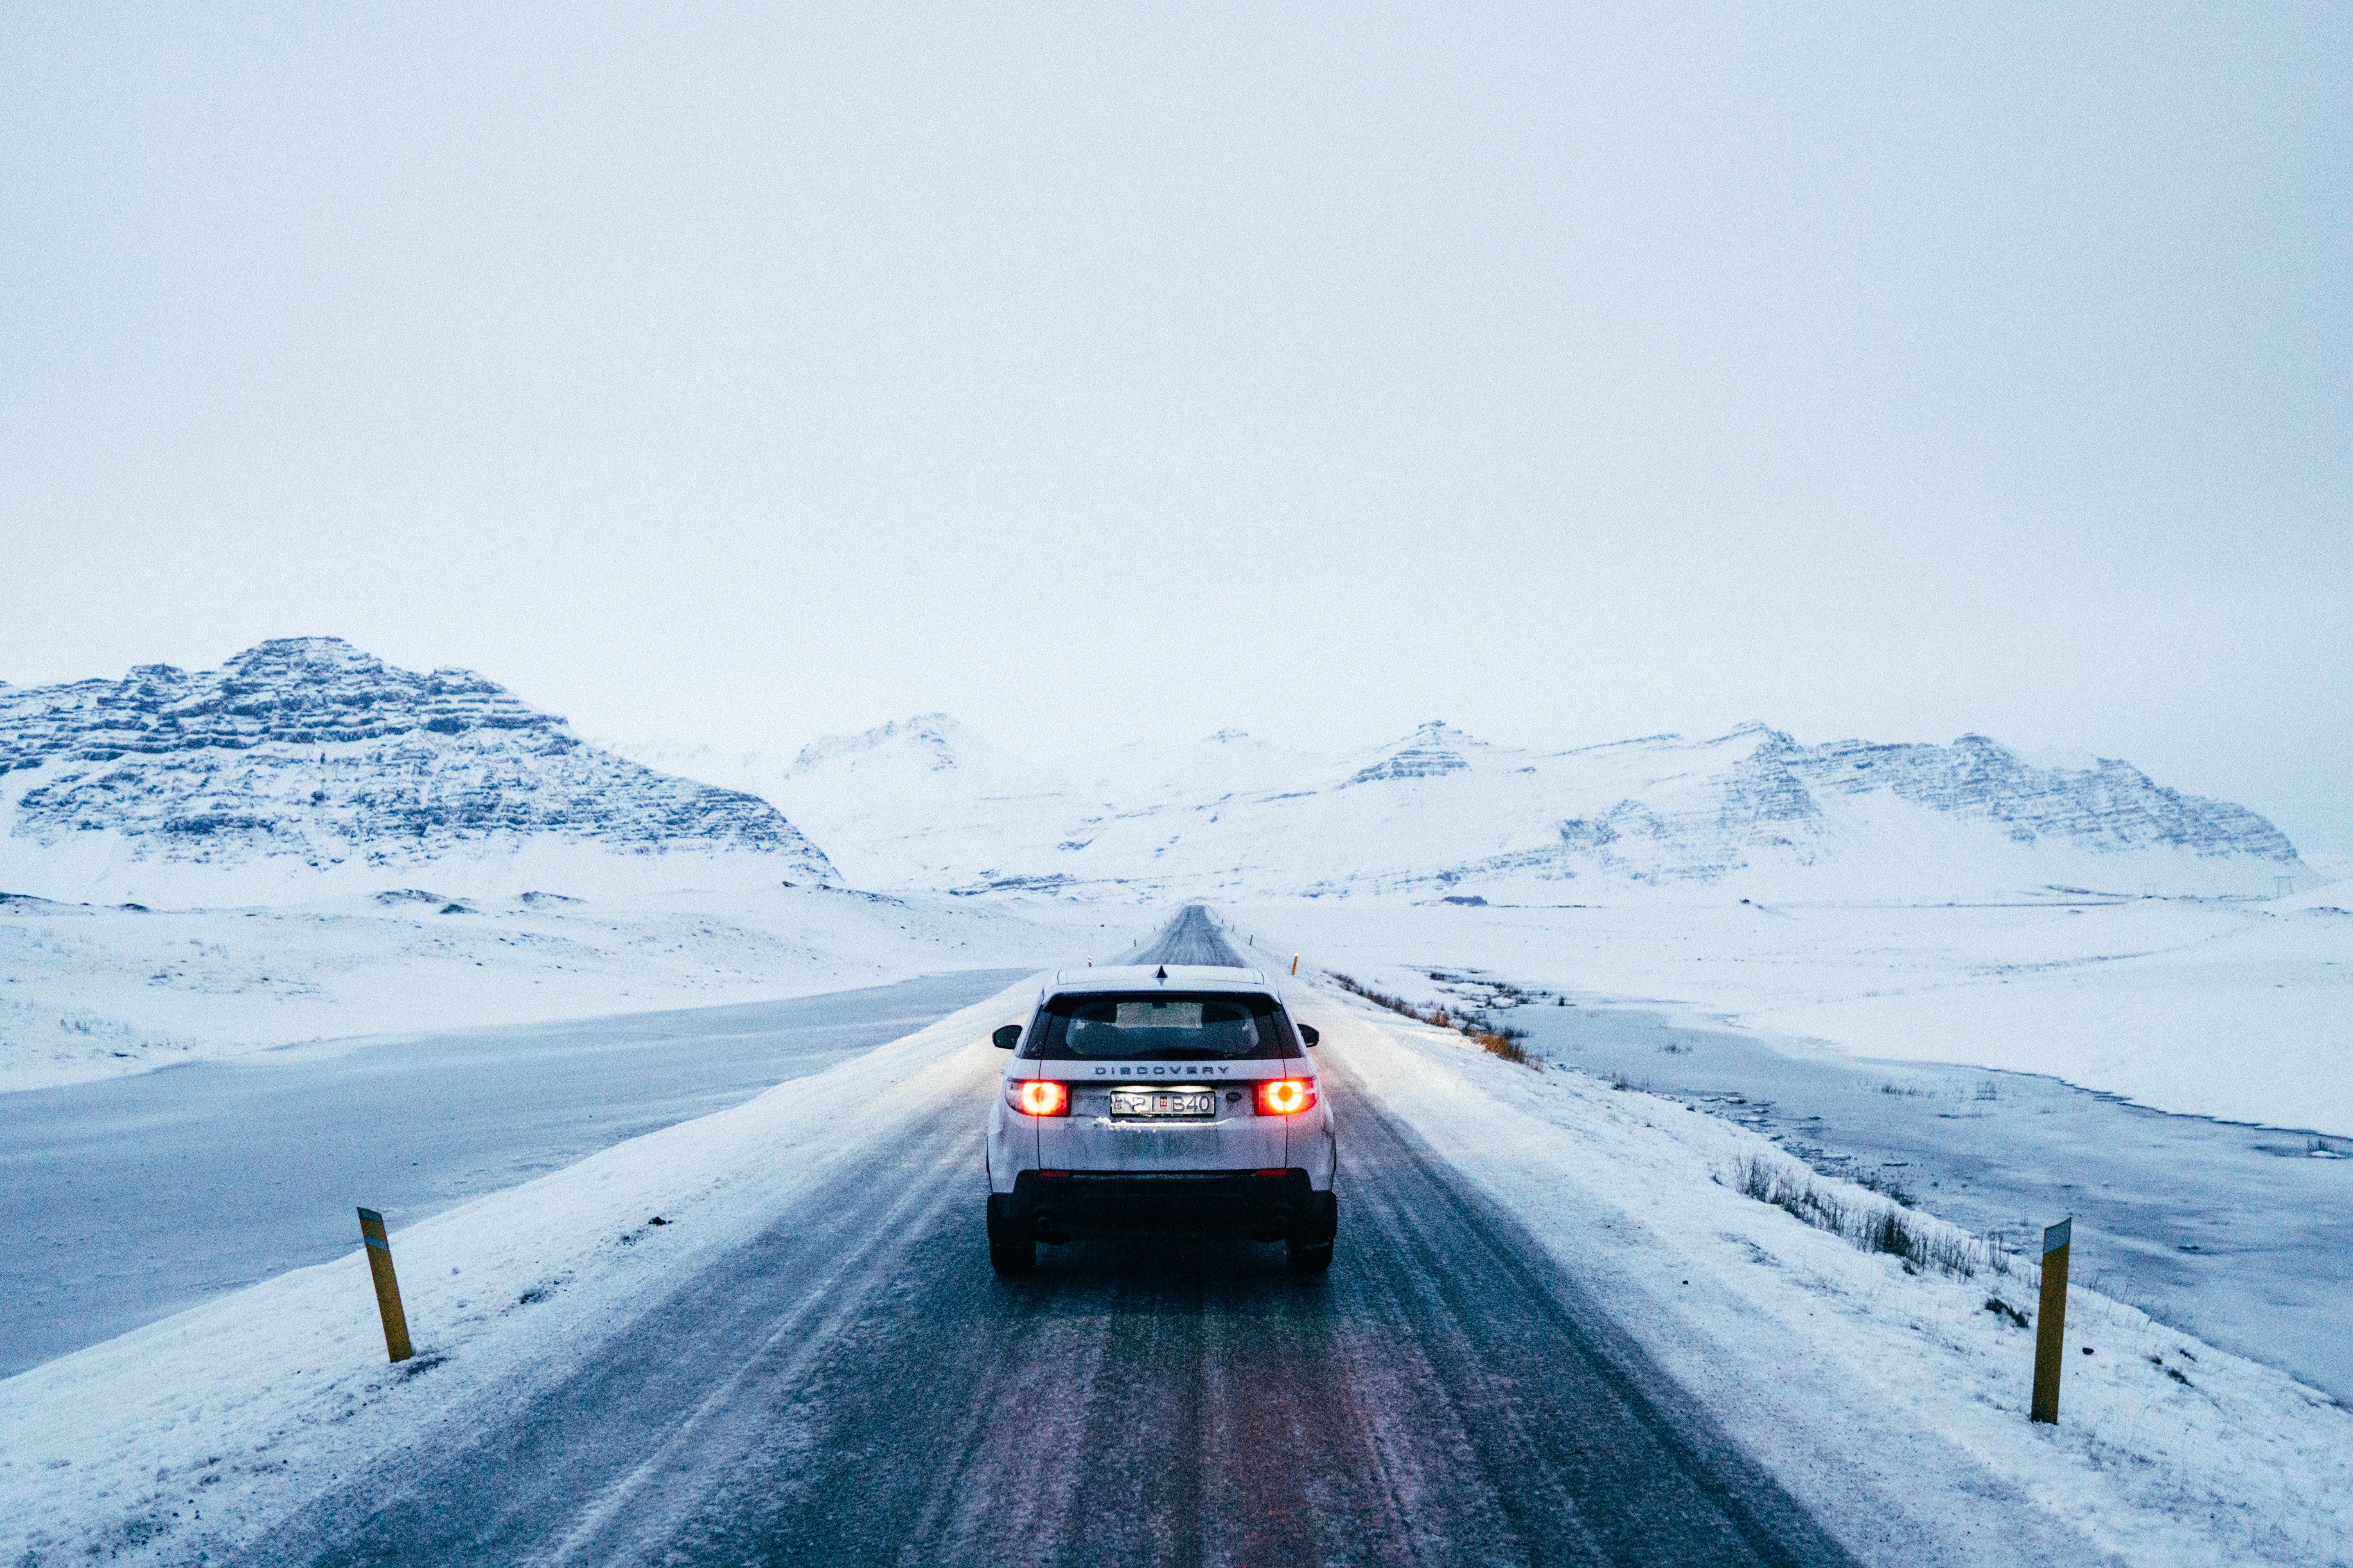
\includegraphics[keepaspectratio=true,scale=0.36]{3.png}} 
		\captionof{figure}{Créer une offre}\label{f3}%
\end{page}
\end{page}





